% !TEX root =  ../Dissertation.tex

\appendix

\chapter{The second universe}
\label{app:etf10}

The regime figures of Chapter~\ref{ch:results} are drawn on \texttt{sector11} and the corresponding \texttt{etf10} numbers are quoted in the text. This appendix shows the \texttt{etf10} counterparts, from the same artifacts. The capacity curve is included here rather than in the main text because its three-seed spreads are too wide to rank the capacities. The error bars in Figure~\ref{fig:app-capacity-etf10} are the evidence for that statement.

\begin{figure}[t]
  \centering
  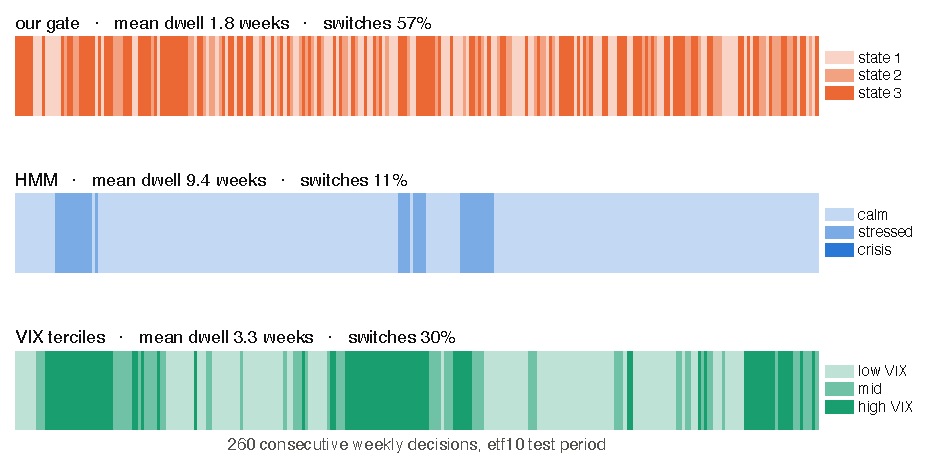
\includegraphics[width=\textwidth]{fig_regime_ribbons_etf10.pdf}
  \caption[Regime timelines, \texttt{etf10}]{Weekly regime labels over five
  consecutive years of the \texttt{etf10} test period. Over the full test
  period the mean dwell times are $1.8$, $9.2$ and $3.3$ weeks for our gate,
  the HMM and the VIX terciles; the same fast-versus-slow pattern as
  \texttt{sector11}.}
  \label{fig:app-ribbons-etf10}
\end{figure}

\begin{figure}[t]
  \centering
  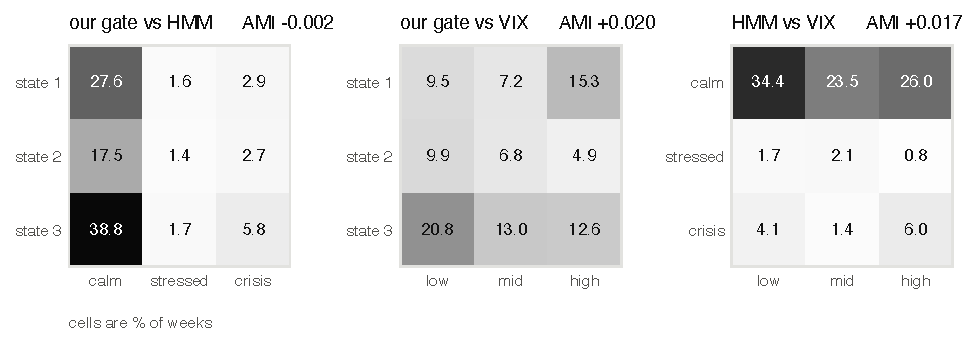
\includegraphics[width=\textwidth]{fig_regime_agreement_etf10.pdf}
  \caption[Regime agreement, \texttt{etf10}]{Co-occurrence of weekly regime
  labels on \texttt{etf10}. Our gate agrees with neither statistical scheme
  (AMI $-0.002$ and $+0.020$). The control pairing is weaker here than on
  \texttt{sector11} ($+0.017$ against $+0.093$), which is why the main text
  claims the clustering of the statistical schemes on one universe only.}
  \label{fig:app-agreement-etf10}
\end{figure}

\begin{figure}[t]
  \centering
  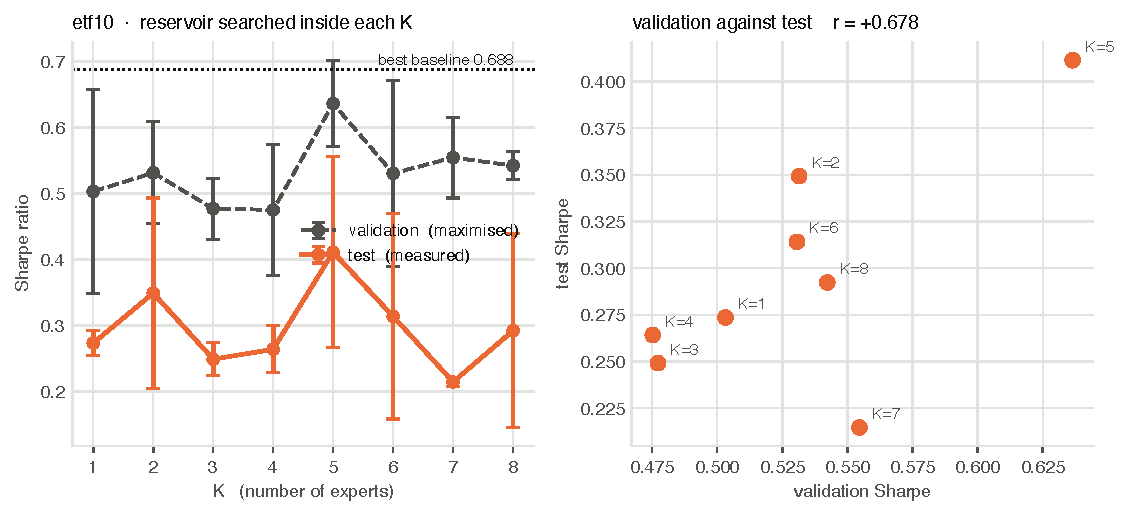
\includegraphics[width=\textwidth]{fig_capacity_curve_etf10.pdf}
  \caption[Capacity curve, \texttt{etf10}]{The withheld \texttt{etf10}
  capacity curve, three seeds per point. The spreads are as large as the
  differences between capacities, and re-running one point at eight seeds
  moved it from $0.215$ to $0.276$ and its spread from $0.007$ to $0.088$, so
  no per-$K$ ordering is read from this curve. Validation and test correlate
  positively here ($r=+0.678$), so the anti-correlation of
  Section~\ref{sec:results-capacity} is a \texttt{sector11} finding, not a
  law.}
  \label{fig:app-capacity-etf10}
\end{figure}

\chapter{Negative results and reversals}
\label{app:negative}

Three results were measured, but kept out of the main text.
They are of lower significance and thus are noted here.
First, a per-date multi-objective selection front (NSGA-II) was built in full on top of the trained blend, measured, and deleted. Restricting the blend to its largest positions costs nothing but re-optimising the positions with the
front destroys performance (Table~\ref{tab:app-nsga}). Bolting a predict-then-optimise step onto the end of a decision-focused system is exactly the pattern the dissertation argues against.

\begin{table}[t]
  \centering
  \begin{tabular}{l rr}
    \hline
    schedule (same model, segment and ledger) & \texttt{etf10} & \texttt{sector11} \\
    \hline
    A: the mixture blend                  & $+0.856$ & $+0.332$ \\
    B: blend restricted to top names      & $+0.909$ & $+0.342$ \\
    C: NSGA-II front on the same names    & $-0.325$ & $-0.231$ \\
    \hline
  \end{tabular}
  \caption[The retired selection front]{One trained model, one validation
  segment, one ledger; only the execution schedule differs.}
  \label{tab:app-nsga}
\end{table}

Second, the price of a tradable book. Keeping only the largest $K_{\text{card}}$
positions and renormalising, with no retraining, costs a measured
$0.08$ of Sharpe (Table~\ref{tab:app-card}).

\begin{table}[t]
  \centering
  \begin{tabular}{l rrrrr}
    \hline
    $K_{\text{card}}$ & 3 & 5 & 7 & 9 & unconstrained \\
    \hline
    Sharpe & 0.546 & 0.588 & 0.637 & 0.663 & \textbf{0.670} \\
    \hline
  \end{tabular}
  \caption[The price of cardinality]{Exact cardinality on the trained blend,
  \texttt{sector11}, $K=1$, twelve folds, five seeds, concatenated
  validation metric. The cost is monotone in tightness.}
  \label{tab:app-card}
\end{table}

Third, the aggregation correction. Early sweeps averaged per-fold Sharpe ratios; Section~\ref{sec:evaluation} explains why that is invalid, and Table~\ref{tab:app-metric} shows it is also material: the two aggregations differ by up to $0.48$ and can reverse a sign. Every number in this dissertation postdates the correction.

\begin{table}[t]
  \centering
  \begin{tabular}{l rr}
    \hline
    same configuration, same folds & mean of folds & concatenated \\
    \hline
    \texttt{sector11}, F01--F03, validation      & $+0.429$ & $-0.053$ \\
    \texttt{etf10}, $K{=}3$, test                & $+0.481$ & $+0.241$ \\
    \texttt{etf10}, single head, test            & $-0.404$ & $+0.310$ \\
    \hline
  \end{tabular}
  \caption[Mean-of-folds against the concatenated metric]{An invalid
  aggregation does not merely shift a number; the last row changes sign.}
  \label{tab:app-metric}
\end{table}

\chapter{Folds and per-year results}
\label{app:folds}

Table~\ref{tab:app-folds} lists every fold. Each fold trains on all data from the universe start (1999 for \texttt{sector11}, 2006 for \texttt{etf10}) to the end of the year before its validation year, less the embargo. Tables~\ref{tab:app-peryear-s11} and~\ref{tab:app-peryear-e10} give the per-year consistency breakdown promised in Section~\ref{sec:evaluation}: one excess Sharpe per test year, computed as the headline metric on the seed-averaged daily streams. A single year holds only $52$ weekly decisions, so these values are noisy by construction and are read for consistency and not as the headline.

\begin{table}[t]
  \centering
  \small
  \begin{minipage}[t]{0.48\textwidth}
    \centering
    \begin{tabular}{lcc}
      \hline
      \texttt{sector11} & validation & test \\
      \hline
      F01 & 2006 & 2007 \\
      F02 & 2007 & 2008 \\
      F03 & 2008 & 2009 \\
      F04 & 2009 & 2010 \\
      F05 & 2010 & 2011 \\
      F06 & 2011 & 2012 \\
      F07 & 2012 & 2013 \\
      F08 & 2013 & 2014 \\
      F09 & 2014 & 2015 \\
      F10 & 2015 & 2016 \\
      F11 & 2016 & 2017 \\
      F12 & 2017 & 2018 \\
      F13 & 2018 & 2019 \\
      F14 & 2019 & 2020 \\
      F15 & 2020 & 2021 \\
      F16 & 2021 & 2022 \\
      F17 & 2022 & 2023 \\
      F18 & 2023 & 2024 \\
      \hline
    \end{tabular}
  \end{minipage}
  \hfill
  \begin{minipage}[t]{0.48\textwidth}
    \centering
    \begin{tabular}{lcc}
      \hline
      \texttt{etf10} & validation & test \\
      \hline
      F01 & 2014 & 2015 \\
      F02 & 2015 & 2016 \\
      F03 & 2016 & 2017 \\
      F04 & 2017 & 2018 \\
      F05 & 2018 & 2019 \\
      F06 & 2019 & 2020 \\
      F07 & 2020 & 2021 \\
      F08 & 2021 & 2022 \\
      F09 & 2022 & 2023 \\
      F10 & 2023 & 2024 \\
      \hline
    \end{tabular}
  \end{minipage}
  \caption[Fold definitions]{The walk-forward folds. Selection used
  F01--F08 (\texttt{sector11}) and F01--F05 (\texttt{etf10}); the held-out
  verification used F13--F18 and F06--F10.}
  \label{tab:app-folds}
\end{table}

\begin{table}[t]
  \centering
  \small
  \begin{tabular}{l rrrrrr}
    \hline
    \texttt{sector11} & 1/N & SPY & inv-vol & LW--MV & $K{=}1$ & $K{=}1$+sig \\
    \hline
    2007 & +0.43 & +0.14 & +0.45 & +0.35 & +0.44 & +0.43 \\
    2008 & -0.88 & -0.85 & -0.91 & -0.50 & -0.96 & -0.98 \\
    2009 & +0.95 & +0.90 & +0.98 & +1.46 & +0.95 & +0.95 \\
    2010 & +0.73 & +0.70 & +0.76 & +0.85 & +0.68 & +0.72 \\
    2011 & +0.22 & +0.15 & +0.32 & -0.17 & +1.34 & +1.34 \\
    2012 & +1.03 & +1.07 & +1.11 & +0.60 & +0.52 & +0.75 \\
    2013 & +2.31 & +2.41 & +2.36 & +2.03 & +2.16 & +2.23 \\
    2014 & +1.31 & +1.29 & +1.40 & +1.18 & +1.29 & +1.29 \\
    2015 & +0.12 & +0.27 & +0.15 & +0.12 & +0.13 & +0.11 \\
    2016 & +1.51 & +1.40 & +1.45 & +0.10 & +0.92 & +1.20 \\
    2017 & +2.52 & +2.64 & +2.64 & +0.71 & +2.41 & +2.40 \\
    2018 & -0.65 & -0.46 & -0.59 & -0.25 & -0.54 & -0.63 \\
    2019 & +2.05 & +2.03 & +2.08 & +1.78 & +0.37 & +1.89 \\
    2020 & +0.45 & +0.64 & +0.50 & +0.28 & +0.41 & +0.41 \\
    2021 & +2.10 & +1.93 & +2.11 & +0.86 & +1.78 & +1.81 \\
    2022 & -0.48 & -0.72 & -0.48 & +0.96 & -0.54 & -0.55 \\
    2023 & +0.76 & +1.38 & +0.57 & +0.41 & +0.74 & +0.70 \\
    2024 & +1.03 & +1.46 & +0.97 & +0.60 & +0.98 & +0.98 \\
    \hline
  \end{tabular}
  \caption[Per-year Sharpe, \texttt{sector11}]{Per-test-year excess Sharpe,
  \texttt{sector11}. $K{=}1$ is the frozen arm; the last column adds the five
  market-level signals.}
  \label{tab:app-peryear-s11}
\end{table}

\begin{table}[t]
  \centering
  \small
  \begin{tabular}{l rrrrrr}
    \hline
    \texttt{etf10} & 1/N & SPY & inv-vol & LW--MV & $K{=}3$ & $K{=}1$+sig \\
    \hline
    2015 & -0.60 & +0.27 & -0.69 & -0.65 & -0.40 & -0.39 \\
    2016 & +1.45 & +1.40 & +1.38 & -1.09 & +1.18 & +1.15 \\
    2017 & +2.38 & +2.64 & +2.31 & +1.16 & +2.29 & +2.28 \\
    2018 & -1.14 & -0.46 & -1.25 & -1.51 & -1.11 & -1.13 \\
    2019 & +2.52 & +2.03 & +2.74 & +0.60 & +2.45 & +2.40 \\
    2020 & +0.67 & +0.64 & +0.61 & +0.07 & +0.59 & +0.59 \\
    2021 & +1.33 & +1.93 & +1.19 & +0.07 & +0.42 & +0.93 \\
    2022 & -1.04 & -0.72 & -1.29 & +0.42 & -1.02 & -1.05 \\
    2023 & +0.28 & +1.38 & +0.17 & +0.04 & +0.24 & +0.37 \\
    2024 & +0.39 & +1.46 & +0.34 & +1.60 & +0.21 & +0.39 \\
    \hline
  \end{tabular}
  \caption[Per-year Sharpe, \texttt{etf10}]{Per-test-year excess Sharpe,
  \texttt{etf10}. $K{=}3$ is the frozen arm; the last column is the single
  head with the five market-level signals.}
  \label{tab:app-peryear-e10}
\end{table}

\chapter{GitLab link}
\label{app:gitlab}

The full project is available at: \url{https://git.cs.bham.ac.uk/projects-2025-26/hxy511}.

\begin{verbatim}
dissertation/
  requirements.txt   pinned packages, Python 3.14
  report/            this document (LaTeX)
  regime-rc/         the project
    src/rrc/         library code: data, reservoir, models, optim,
                     backtest, baselines, eval, utils
    scripts/         one entry point per experiment (run_*.py)
                     and per figure (make_*_figures.py)
    configs/         YAML configurations; configs/frozen/ holds
                     the frozen defaults
    tests/           pytest suite (make test)
    results/         append-only registry.csv, runs and figures
    Makefile         every pipeline step as a copy-paste recipe
\end{verbatim}

There are two extra folders seen in gitlab as well being portfolio-data and portfolio-forecast, they were done as initial testing and not important for this report. To run: create a virtual environment, install \texttt{requirements.txt}, and
work from inside \texttt{regime-rc/}. \texttt{make data} builds the data
artifacts (cached locally, offline after the first pull), \texttt{make test}
runs the test suite, and the remaining targets in the \texttt{Makefile} map
one-to-one onto the experiments of Chapter~\ref{ch:results}. Every
\texttt{run\_*.py} script requires \texttt{--universe etf10} or
\texttt{--universe sector11}. The one exception to re-running is
\texttt{scripts/run\_holdout.py}, which was run exactly once by design and
should not be run again.
